%% Machine Learning and Agentic AI for Macroeconomic Research
%% Lecture 8: Retrieval Augmented Generation (RAG)
%% Author: Zhigang Feng

\documentclass[10pt,english,aspectratio=169]{beamer}

\usepackage{ae,aecompl}
\usepackage[T1]{fontenc}
\usepackage{textcomp}
\usepackage[utf8]{inputenc}
\usepackage{babel}

\setcounter{secnumdepth}{3}
\setcounter{tocdepth}{3}

\usepackage{amsmath, amssymb, graphicx}
\usepackage{booktabs, multirow}
\usepackage{tikz}
\usetikzlibrary{arrows.meta, positioning, shapes.geometric, fit, calc, backgrounds}
\usepackage{listings}
\usepackage{xcolor}

\lstset{
  basicstyle=\ttfamily\small,
  keywordstyle=\color{blue!80!black}\bfseries,
  commentstyle=\color{green!50!black}\itshape,
  stringstyle=\color{orange!80!black},
  backgroundcolor=\color{gray!8},
  frame=single,
  rulecolor=\color{gray!40},
  breaklines=true,
  showstringspaces=false,
  numbers=none,
}

\ifx\hypersetup\undefined
  \AtBeginDocument{%
    \hypersetup{bookmarks=false,breaklinks=true,pdfborder={0 0 0},colorlinks=true,
      linkcolor=DarkText,urlcolor=RedTitle}%
  }
\else
  \hypersetup{bookmarks=false,breaklinks=true,pdfborder={0 0 0},colorlinks=true,
    linkcolor=DarkText,urlcolor=RedTitle}%
\fi

\makeatletter
\newcommand\makebeamertitle{\frame{\maketitle}}%
\AtBeginDocument{%
  \let\origtableofcontents=\tableofcontents
  \def\tableofcontents{\@ifnextchar[{\origtableofcontents}{\gobbletableofcontents}}
  \def\gobbletableofcontents#1{\origtableofcontents}%
}

\usetheme{metropolis}
\usefonttheme{professionalfonts}

\definecolor{LightGray}{RGB}{230,230,230}
\definecolor{RedTitle}{RGB}{0,0,200}
\definecolor{VeryLightGray}{RGB}{245,245,245}
\definecolor{DarkText}{RGB}{0,0,0}

\setbeamercolor{background canvas}{bg=white}
\setbeamercolor{title}{fg=RedTitle}
\setbeamercolor{author}{fg=DarkText}
\setbeamercolor{date}{fg=DarkText}
\setbeamercolor{frametitle}{bg=VeryLightGray,fg=DarkText}
\setbeamercolor{normal text}{fg=DarkText}

\setbeamersize{text margin left=5mm, text margin right=5mm}
\addtobeamertemplate{frametitle}{}{\vspace{-0.5em}}
\newcommand{\reducevspace}{\vspace{-0.5cm}}

\setbeamertemplate{navigation symbols}{}
\setbeamertemplate{footline}{%
  \hfill%
  \usebeamercolor[fg]{page number in head/foot}%
  \usebeamerfont{page number in head/foot}%
  \insertframenumber\,/\,\inserttotalframenumber\kern1em\vskip2pt%
}

\makeatother

\graphicspath{{figures/}}

\title[ML \& Agentic AI for Macro Research]{Machine Learning and Agentic AI for Macroeconomic Research\\
8: Retrieval Augmented Generation (RAG)\\[0.5em]}
\author{Zhigang Feng}
\date{Spring 2026}

\begin{document}

\makebeamertitle

%=============================================================================
% AGENDA
%=============================================================================

\begin{frame}{Lecture Agenda}
\begin{enumerate}
  \item \textbf{From LLMs to RAG} --- knowledge cutoffs, hallucinations, why static models fall short
  \medskip
  \item \textbf{The Naive Approach} --- prompt engineering and why it hits a wall
  \medskip
  \item \textbf{An Intuition First} --- personal wiki knowledge bases (Karpathy, 2025)
  \medskip
  \item \textbf{RAG: The Principled Solution} --- separating indexing from querying
  \medskip
  \item \textbf{Step 1 --- Document Ingestion \& Chunking}
  \medskip
  \item \textbf{Step 2 --- Embeddings} --- text as geometry
  \medskip
  \item \textbf{Step 3 --- Vector Storage \& Retrieval}
  \medskip
  \item \textbf{Beyond Dense Retrieval} --- graph-based and hierarchical RAG
  \medskip
  \item \textbf{Step 4 --- Augmented Generation} --- prompt templates, attribution, faithfulness
  \medskip
  \item \textbf{RAG vs.\ Fine-Tuning} --- when to use which
  \medskip
  \item \textbf{Applications in Economic Research} --- FOMC, NBER, Congress, SEC, central banks
  \medskip
  \item \textbf{Limitations, Failure Modes \& Evaluation}
  \medskip
  \item \textbf{Bridge to Lec.\ 9} --- from single-shot RAG to agentic research
\end{enumerate}
\end{frame}

%=============================================================================
\section{Where We Are}
% PART I: WHERE WE ARE -- FROM LLMs TO RAG
%=============================================================================

\begin{frame}{Recap: What an LLM Is (Lecture 7)}
\begin{itemize}
\item A \textbf{Large Language Model} is a neural network that maps a sequence of tokens to a probability distribution over the next token.

\medskip
\item \textbf{Pipeline:} Tokenization $\to$ Token embeddings $\to$ Transformer layers (attention + feed-forward) $\to$ Output distribution.

\medskip
\item \textbf{Knowledge is parametric:} Everything the model ``knows'' is encoded in its weights, frozen at the end of pretraining.

\medskip
\item \textbf{Implication:} The model has no memory beyond its weights and the current context window. Once training is over, its knowledge of the world is fixed in time.

\medskip
\item \textbf{Today's question:} How do we extend that knowledge \emph{at inference time}, without retraining?
\end{itemize}
\end{frame}

\begin{frame}{What an LLM Knows vs.\ What It Can Know}
\begin{itemize}
\item Every LLM has a \textbf{knowledge cutoff}: the date when its training corpus stopped.
\begin{itemize}
    \item GPT-4 Turbo: April 2023
    \item GPT-4o: October 2023
    \item Claude 3.5 Sonnet: April 2024
    \item Claude 4 Opus: early 2025
\end{itemize}

\medskip
\item \textbf{Concrete problem:} Ask the model: \emph{``What did the FOMC decide at its December 2025 meeting?''}
\begin{itemize}
    \item A pre-2025 model has \emph{never seen} the December 2025 statement.
    \item It will either refuse, or worse, \emph{hallucinate} a plausible but fictional answer.
\end{itemize}

\medskip
\item \textbf{The economist's view:} Macro and finance research depends on the latest data. A model that can't read the December press release is not a research tool.

\medskip
\item \textbf{Even within the cutoff:} Private datasets (your own working papers, internal Fed memos, FOIA-released records) were never in the training corpus at all.
\end{itemize}
\end{frame}

\begin{frame}{Three Pain Points for the Economist}
\begin{itemize}
\item \textbf{1. Stale knowledge.} Anything published after the cutoff is invisible. So is anything proprietary.

\medskip
\item \textbf{2. Hallucinated citations.} A vanilla LLM asked to ``cite five NBER papers on the slope of the Phillips curve'' will happily produce five plausible titles, plausible authors, and entirely fake DOIs. This is the most common failure mode in academic use.

\medskip
\item \textbf{3. No source attribution.} Even when the answer is correct, the model cannot tell you \emph{where} the claim came from. Academic research requires footnotes.

\medskip
\item \textbf{Bottom line:} For research-grade work we need a system that can (i) read documents the model never saw, (ii) refuse to invent facts, and (iii) tell us which document supplied each claim.
\end{itemize}
\end{frame}

\begin{frame}{Two Ways to Add Knowledge}
\begin{itemize}
\item \textbf{Option A --- Fine-Tuning:} Re-train (some of) the model's weights on your new corpus.
\begin{itemize}
    \item Pros: knowledge becomes ``baked in,'' fast at inference.
    \item Cons: expensive, fragile, hard to update, no source attribution, doesn't fix hallucination.
\end{itemize}

\medskip
\item \textbf{Option B --- Retrieval (RAG):} Leave the model untouched. At query time, fetch the relevant text from an external store and \emph{paste it into the prompt}.
\begin{itemize}
    \item Pros: cheap, updatable in real time, gives source attribution, dramatically reduces hallucination.
    \item Cons: more moving parts; quality depends on the retriever.
\end{itemize}

\medskip
\item \textbf{Promise of this lecture:} By the end you will understand both options, know when to use each, and have seen the full RAG pipeline applied to FOMC and NBER corpora.

\medskip
\item \textbf{Detailed comparison:} Section VIII.
\end{itemize}
\end{frame}

%=============================================================================
\section{Naive Prompt Engineering Alone}
% PART II: THE NAIVE APPROACH -- PROMPT ENGINEERING ALONE
%=============================================================================

\begin{frame}{What Is ``Naive Prompt Engineering''?}
\begin{itemize}
\item \textbf{Definition:} The simplest possible workaround for the knowledge-cutoff problem --- paste your documents \emph{directly} into the prompt and ask a question.

\medskip
\item \textbf{Tiny example:}
\begin{quote}
\small
\textit{``Here is the December 2025 FOMC statement:\\
{[paste full text of statement]}\\
Question: What did the Committee say about inflation expectations?''}
\end{quote}

\medskip
\item This \emph{is} how most economists first try to use ChatGPT/Claude on real data. It works for tiny inputs and feels natural.

\medskip
\item \textbf{Why we start here:} If naive prompt engineering scaled, RAG would be unnecessary. We need to understand precisely \emph{where} it breaks before introducing the principled fix.
\end{itemize}
\end{frame}

\begin{frame}{A Tempting First Attempt}
\begin{itemize}
\item \textbf{Research question:} \emph{``How did the FOMC's framing of inflation expectations evolve from 2020 to 2025?''}

\medskip
\item \textbf{Naive plan:} Download every FOMC statement and minutes file from 2020 through 2025, concatenate them, paste the result into one giant prompt, and ask the question.

\medskip
\item \textbf{Schematic prompt:}
\begin{quote}
\small
\texttt{[2020-Jan minutes] [2020-Mar statement] [2020-Apr minutes] \dots\\
\dots [2025-Dec statement]\\
Question: How did the framing of inflation expectations evolve from 2020 to 2025?}
\end{quote}

\medskip
\item In principle this should work --- the model has all the data it needs. \textbf{In practice this fails for at least four reasons.} We will tour them next.
\end{itemize}
\end{frame}

\begin{frame}{Limit \#1: The Context Window}
\begin{itemize}
\item Every LLM has a hard cap on how many tokens it can read at once --- the \textbf{context window}.
\begin{itemize}
    \item Claude 4 Opus: 200{,}000 tokens (about 150{,}000 English words)
    \item GPT-4 Turbo: 128{,}000 tokens
    \item Gemini 1.5 Pro: 1{,}000{,}000 tokens (rare, expensive)
\end{itemize}

\medskip
\item \textbf{How big is the FOMC corpus?}
\begin{itemize}
    \item 8 meetings per year $\times$ statement ($\sim$1{,}000 tokens) + minutes ($\sim$15{,}000 tokens) + transcript ($\sim$100{,}000 tokens, released with 5-year lag)
    \item Conservative estimate \emph{excluding} transcripts: $\sim$130{,}000 tokens \emph{per year}
    \item Five years (2020--2024): $\sim$650{,}000 tokens
\end{itemize}

\medskip
\item \textbf{Verdict:} Five years of FOMC text \emph{does not fit} in any model's context window. And we haven't even added press conferences, speeches, or Beige Books.

\medskip
\item \textbf{This is a hard wall, not a tuning parameter.}
\end{itemize}
\end{frame}

\begin{frame}{Limit \#2: Cost}
\begin{itemize}
\item Even when content fits, you pay for \emph{every input token, every query.}

\medskip
\item \textbf{Pricing as of 2025} (Anthropic + OpenAI public rates):
\begin{itemize}
    \item Claude 4 Opus input: \$15 / million tokens
    \item GPT-4o input: \$2.50 / million tokens
\end{itemize}

\medskip
\item \textbf{Cost arithmetic:} Suppose you stuff 600K tokens of FOMC text into each query.
\begin{itemize}
    \item One query on Opus: $0.6 \times \$15 = \$9.00$
    \item One query on GPT-4o: $0.6 \times \$2.50 = \$1.50$
    \item One thousand exploratory queries: \$9{,}000 / \$1{,}500
\end{itemize}

\medskip
\item \textbf{And:} You pay this \emph{every time}, even if you ask the same question twice. There's no caching of expensive context across sessions.

\medskip
\item \textbf{For research:} Prohibitive at the scale of an actual literature review or empirical project.
\end{itemize}
\end{frame}

\begin{frame}{Limit \#3: Latency and ``Lost in the Middle''}
\begin{itemize}
\item Long contexts are \textbf{slow}. Inference time grows roughly linearly (or worse) in input token count. A 600K-token query can take 30+ seconds before the first response token.

\medskip
\item \textbf{Worse:} Performance \emph{degrades} as context grows. Liu et al.\ (2024), \emph{``Lost in the Middle: How Language Models Use Long Contexts''}:
\begin{itemize}
    \item Models attend strongly to the \emph{start} and \emph{end} of the context.
    \item Information \emph{in the middle} is systematically missed.
    \item The accuracy curve as a function of relevant-document position is U-shaped.
\end{itemize}

\medskip
\item \textbf{Implication for the FOMC example:} Even if the December 2025 statement \emph{did} fit, it would land in the middle of your concatenated corpus and the model would likely under-weight it.

\medskip
\item \textbf{Punchline:} Cramming everything into the prompt does not just cost more --- it actually \emph{hurts} answer quality.
\end{itemize}
\end{frame}

\begin{frame}{Limit \#4: No Scalability or Persistence}
\begin{itemize}
\item Naive prompt engineering treats every query as a \textbf{fresh start}.
\begin{itemize}
    \item No reuse of work across queries.
    \item No incremental updates when the Fed releases new minutes next month.
    \item No way to grow the corpus past the context window --- ever.
\end{itemize}

\medskip
\item \textbf{Compare to a real research workflow:}
\begin{itemize}
    \item You collect documents \emph{once}.
    \item You index them \emph{once}.
    \item You ask many questions over time, paying only for what you actually retrieve.
    \item When new documents arrive, you index them incrementally.
\end{itemize}

\medskip
\item Naive prompt engineering supports \emph{none} of this. Every question is a brand-new copy-paste.

\medskip
\item \textbf{The pattern we need:} Separate the cost of \emph{ingesting documents} from the cost of \emph{asking questions}.
\end{itemize}
\end{frame}

\begin{frame}{The Wall}
\begin{center}
\renewcommand{\arraystretch}{1.4}
\begin{tabular}{|p{5.5cm}|p{8cm}|}
\hline
\textbf{Naive prompt engineering can do} & \textbf{Research workflows actually need} \\
\hline
QA on a single short document & QA over millions of tokens of corpus \\
\hline
Tens of queries before cost bites & Thousands of queries over weeks \\
\hline
Whatever fits in 200K tokens & Decades of FOMC + NBER + 10-K filings \\
\hline
Today's prompt only & Incremental updates as new docs arrive \\
\hline
``Trust me'' answers & Cited, source-attributed answers \\
\hline
\end{tabular}
\end{center}

\bigskip
\textbf{Conclusion:} Prompt engineering hits a hard wall on freshness, scale, latency, cost, and attribution. We need a fundamentally different architecture --- one that \textbf{separates indexing from querying}.

\bigskip
\centering\emph{This is what RAG does.}
\end{frame}

%=============================================================================
\section{Before the Formalism: Personal Wiki Knowledge Bases}
% INTERLUDE: AN INTUITION VIA KARPATHY'S LLM WIKI
%=============================================================================

\begin{frame}{Before the Formalism: A Personal Wiki}
\begin{itemize}
\item Before we build the full RAG pipeline, consider a \textbf{simpler version} of the same idea that you can set up today.

\medskip
\item \textbf{Andrej Karpathy} (June 2025):
\begin{quote}
\small\itshape
``I'm finding very useful recently: using LLMs to build personal knowledge bases for various topics of research interest. \textnormal{[\ldots]} A large fraction of my recent token throughput is going less into manipulating code, and more into \textbf{manipulating knowledge} (stored as markdown and images).''
\end{quote}

\medskip
\item \textbf{The workflow is disarmingly simple:}
\begin{enumerate}
    \item Collect source documents (papers, articles, data) into a \texttt{raw/} directory.
    \item Ask an LLM to \emph{compile} them into a \textbf{wiki} --- a directory of \texttt{.md} files with summaries, concept articles, and cross-links.
    \item Query the wiki by asking the LLM questions; it reads the relevant articles and answers from them.
\end{enumerate}

\medskip
\item \textbf{Why this matters for us:} This is the \emph{same core insight} behind RAG --- separating data ingestion from querying --- but without any of the formal machinery.
\end{itemize}
\end{frame}

\begin{frame}{The Wiki Pipeline}
\begin{center}
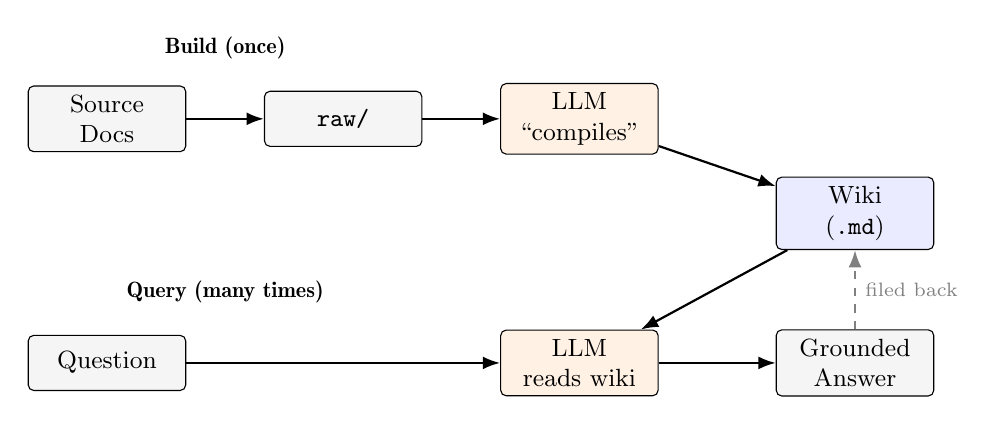
\begin{tikzpicture}[
  font=\small,
  box/.style={draw, rounded corners=2pt, minimum width=2.0cm, minimum height=0.7cm, align=center, fill=VeryLightGray},
  llm/.style={draw, rounded corners=2pt, minimum width=2.0cm, minimum height=0.7cm, align=center, fill=orange!10},
  store/.style={draw, rounded corners=2pt, minimum width=2.0cm, minimum height=0.8cm, align=center, fill=blue!8},
  arr/.style={-{Latex[length=2.2mm]}, thick},
  darr/.style={-{Latex[length=2.2mm]}, thick, dashed, gray}
]
  % Build phase (top row)
  \node[font=\footnotesize\bfseries] at (1.5, 2.3) {Build (once)};
  \node[box] (docs) at (0, 1.4) {Source\\Docs};
  \node[box] (raw) at (3, 1.4) {\texttt{raw/}};
  \node[llm] (llm1) at (6, 1.4) {LLM\\``compiles''};

  % Wiki (shared artifact)
  \node[store] (wiki) at (9.5, 0.2) {Wiki\\(\texttt{.md})};

  % Query phase (bottom row)
  \node[font=\footnotesize\bfseries] at (1.5, -0.8) {Query (many times)};
  \node[box] (q) at (0, -1.7) {Question};
  \node[llm] (llm2) at (6, -1.7) {LLM\\reads wiki};
  \node[box] (ans) at (9.5, -1.7) {Grounded\\Answer};

  \draw[arr] (docs) -- (raw);
  \draw[arr] (raw) -- (llm1);
  \draw[arr] (llm1) -- (wiki);
  \draw[arr] (q) -- (llm2);
  \draw[arr] (wiki) -- (llm2);
  \draw[arr] (llm2) -- (ans);

  % Feedback loop: answers filed back into wiki
  \draw[darr] (ans.north) -- node[right, font=\scriptsize, text=gray] {filed back} (wiki.south);
\end{tikzpicture}
\end{center}

\medskip
\begin{itemize}
\item \textbf{Data ingest:} Download papers, clip web articles, save datasets $\to$ \texttt{raw/}.
\item \textbf{Compile:} LLM reads raw data, produces wiki articles --- summaries, concept pages, back-links. \emph{You rarely edit the wiki manually; the LLM maintains it.}
\item \textbf{Query:} Ask the LLM a question. It reads the wiki's index and relevant articles, then answers with grounded citations.
\item \textbf{Feedback loop (dashed):} Answers and explorations get filed \emph{back} into the wiki, so your research ``adds up'' instead of disappearing after each chat.
\end{itemize}
\end{frame}

\begin{frame}{Wiki vs.\ RAG: Same Intuition, Different Scale}
\begin{center}
\renewcommand{\arraystretch}{1.3}
\begin{tabular}{|p{3.0cm}|p{4.5cm}|p{5.5cm}|}
\hline
& \textbf{Personal Wiki} & \textbf{Full RAG Pipeline} \\
\hline
\textbf{Ingestion} & LLM reads raw docs, writes \texttt{.md} summaries & Chunk $\to$ embed $\to$ store in vector DB \\
\hline
\textbf{``Retrieval''} & LLM reads index files, picks relevant articles & Embedding similarity search (top-$K$) \\
\hline
\textbf{Generation} & LLM answers from wiki articles in context & LLM answers from retrieved chunks \\
\hline
\textbf{Scale limit} & ${\sim}$400K words (must fit in context) & Millions of tokens (no upper limit) \\
\hline
\textbf{Update} & LLM rewrites/extends articles & Add new chunks incrementally \\
\hline
\textbf{Attribution} & Article titles and links & Chunk IDs and source metadata \\
\hline
\end{tabular}
\end{center}

\medskip
\begin{itemize}
\item Karpathy: \emph{``I thought I had to reach for fancy RAG, but the LLM has been pretty good about auto-maintaining index files and brief summaries \textnormal{[\ldots]} at this $\sim$small scale.''}

\medskip
\item \textbf{The wiki \emph{is} retrieval} --- just LLM-curated rather than automated via embeddings. Both architectures solve the same problem: \textbf{separating ingestion from querying}.
\end{itemize}
\end{frame}

\begin{frame}[fragile]{Hands-On: A Mini Wiki for This Course}
\begin{lstlisting}[basicstyle=\ttfamily\footnotesize]
course_wiki/
  index.md                  -- master table of contents
  concepts/
    embeddings.md           -- text-to-vector mappings (Lec 7-8)
    rag.md                  -- retrieval augmented generation
    transformers.md         -- the architecture behind LLMs
  lectures/
    lec07_llm.md            -- key ideas from Lecture 7
    lec08_rag.md            -- key ideas from Lecture 8
  papers/
    vaswani_2017.md         -- Attention Is All You Need
    lewis_2020_rag.md       -- RAG original paper (NeurIPS)
  connections/
    cross_references.md     -- links across lectures
\end{lstlisting}

\medskip
\begin{itemize}
\item A student asks: \emph{``How do the embeddings from Lecture 7 connect to vector stores in Lecture 8?''} --- the LLM reads the relevant wiki pages and gives a \textbf{grounded, cross-referenced} answer.
\item As the course progresses, \textbf{every new lecture enriches the wiki}. Your questions ``add up'' instead of disappearing after each chat session.
\item \textbf{See \texttt{wiki\_demo/}} in the lecture folder for a working example you can browse and extend.
\end{itemize}
\end{frame}

\begin{frame}{From Wiki to RAG: Why We Need the Formal Machinery}
\begin{itemize}
\item The personal wiki works beautifully \textbf{at small scale}: ${\sim}$100 articles, ${\sim}$400K words. A modern LLM can read the whole index plus relevant articles in one context window.

\medskip
\item \textbf{But our economics corpora are much larger:}
\begin{itemize}
    \item 30 years of FOMC minutes + transcripts: millions of tokens
    \item NBER working paper archive: tens of thousands of papers
    \item Congressional Record: billions of words
\end{itemize}

\medskip
\item \textbf{The progression is natural:}
\begin{enumerate}
    \item \textbf{Naive prompting} (paste docs into the prompt) $\to$ hits context window at ${\sim}$200K tokens
    \item \textbf{Personal wiki} (LLM-curated summaries) $\to$ hits context window at ${\sim}$400K words
    \item \textbf{RAG} (vector search over embeddings) $\to$ scales to millions of documents
\end{enumerate}

\medskip
\item Each step is a natural response to the \textbf{scaling problem}. RAG is the wiki idea \emph{formalized and automated}: instead of an LLM maintaining an index by hand, we use embeddings and similarity search to do retrieval at arbitrary scale.

\medskip
\item Karpathy: \emph{``I think there is room here for an incredible new product instead of a hacky collection of scripts.''}
\end{itemize}
\end{frame}

%=============================================================================
\section{RAG --- The Principled Solution}
% PART III: RAG -- THE PRINCIPLED SOLUTION
%=============================================================================

\begin{frame}{The Key Insight}
\begin{itemize}
\item Don't paste the whole corpus into every prompt.

\medskip
\item Instead:
\begin{enumerate}
    \item \textbf{Pre-process documents once.} Split them into chunks, convert each chunk to a numerical fingerprint (an \emph{embedding}), store everything in a database.
    \item \textbf{At query time, fetch only what's relevant.} Convert the user's question to an embedding, look up the closest chunks in the database, paste \emph{those few chunks} into the prompt.
    \item \textbf{Let the LLM answer from the retrieved evidence}, citing which chunks it used.
\end{enumerate}

\medskip
\item This is a \textbf{two-phase architecture:}
\begin{itemize}
    \item \emph{Offline:} index everything once.
    \item \emph{Online:} retrieve a few relevant pieces per query, generate the answer.
\end{itemize}

\medskip
\item Cost is now proportional to \emph{what you actually need}, not to the size of the corpus. Storage is amortized. Indexes are updatable. The model only ever sees relevant text, so quality and faithfulness improve.
\end{itemize}
\end{frame}

\begin{frame}{Definition}
\begin{itemize}
\item \textbf{Retrieval Augmented Generation (RAG):}\\
A system that, before answering a query, \emph{retrieves} relevant documents from an external knowledge store and supplies them to a language model as additional context for \emph{generation}.

\medskip
\item \textbf{Origin:} Lewis, Perez, Piktus, et al.\ (2020), \emph{``Retrieval-Augmented Generation for Knowledge-Intensive NLP Tasks,''} NeurIPS.

\medskip
\item Originally framed as a research architecture for open-domain QA. Now the \emph{de facto} production pattern for any LLM application that touches a custom knowledge base: customer-support bots, legal research, medical Q\&A, code search, and academic research.

\medskip
\item \textbf{Key idea (worth repeating):} The LLM is the \emph{reasoner}. The vector store is the \emph{memory}. The retriever is the \emph{librarian}. RAG is how we connect them.
\end{itemize}
\end{frame}

\begin{frame}{End-to-End Architecture}
\begin{center}
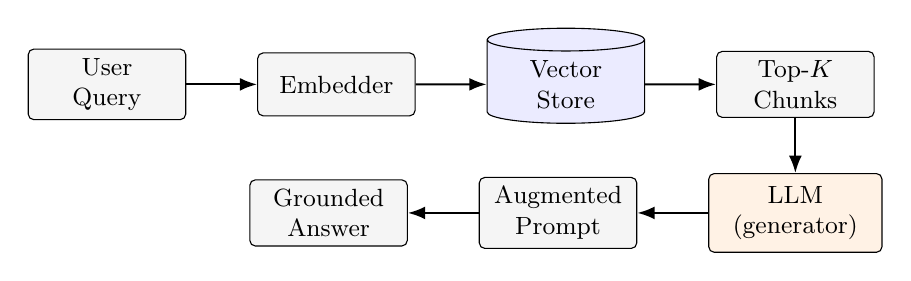
\begin{tikzpicture}[
  font=\small,
  node distance=0.7cm and 0.9cm,
  box/.style={draw, rounded corners=2pt, minimum width=2.0cm, minimum height=0.8cm, align=center, fill=VeryLightGray},
  store/.style={draw, cylinder, shape border rotate=90, aspect=0.25, minimum width=2.0cm, minimum height=1.1cm, align=center, fill=blue!8},
  llm/.style={draw, rounded corners=2pt, minimum width=2.2cm, minimum height=1.0cm, align=center, fill=orange!10},
  arr/.style={-{Latex[length=2.2mm]}, thick}
]
  \node[box] (q) {User\\Query};
  \node[box, right=of q] (emb) {Embedder};
  \node[store, right=of emb] (db) {Vector\\Store};
  \node[box, right=of db] (top) {Top-$K$\\Chunks};
  \node[llm, below=of top] (llm) {LLM\\(generator)};
  \node[box, left=of llm] (ctx) {Augmented\\Prompt};
  \node[box, left=of ctx] (ans) {Grounded\\Answer};

  \draw[arr] (q) -- (emb);
  \draw[arr] (emb) -- (db);
  \draw[arr] (db) -- (top);
  \draw[arr] (top) -- (llm);
  \draw[arr] (llm) -- (ctx);
  \draw[arr] (ctx) -- (ans);
\end{tikzpicture}
\end{center}

\medskip
\textbf{Five components:}
\begin{enumerate}
\item \textbf{Embedder} --- maps text to vectors (Section V).
\item \textbf{Vector store} --- holds embeddings of every chunk (Section VI).
\item \textbf{Retriever} --- pulls the top-$K$ closest chunks to the query.
\item \textbf{Augmented prompt} --- retrieved chunks + user question + instructions (Section VII).
\item \textbf{Generator} --- the LLM that writes the final answer.
\end{enumerate}
\end{frame}

\begin{frame}{Two Phases --- Offline Indexing}
\begin{center}
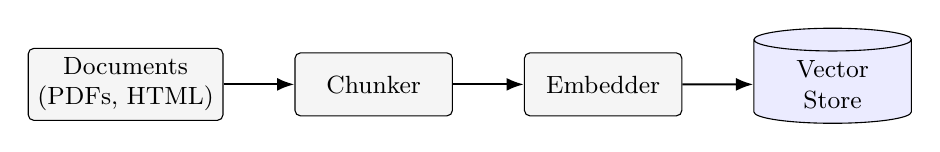
\begin{tikzpicture}[
  font=\small,
  node distance=0.6cm and 0.9cm,
  box/.style={draw, rounded corners=2pt, minimum width=2.0cm, minimum height=0.8cm, align=center, fill=VeryLightGray},
  store/.style={draw, cylinder, shape border rotate=90, aspect=0.25, minimum width=2.0cm, minimum height=1.1cm, align=center, fill=blue!8},
  arr/.style={-{Latex[length=2.2mm]}, thick}
]
  \node[box] (docs) {Documents\\(PDFs, HTML)};
  \node[box, right=of docs] (chunk) {Chunker};
  \node[box, right=of chunk] (emb) {Embedder};
  \node[store, right=of emb] (db) {Vector\\Store};

  \draw[arr] (docs) -- (chunk);
  \draw[arr] (chunk) -- (emb);
  \draw[arr] (emb) -- (db);
\end{tikzpicture}
\end{center}

\medskip
\begin{itemize}
\item Done \textbf{once} --- or incrementally as new documents arrive.
\item Cost is paid up front; queries are then cheap.
\item \textbf{Library catalog analogy:} Building the card catalog is slow work. Once it exists, looking things up is fast.
\item \textbf{For an economist:} Index the entire FOMC archive (1993--present) one weekend; then query it for years.
\end{itemize}
\end{frame}

\begin{frame}{Two Phases --- Online Query}
\begin{center}
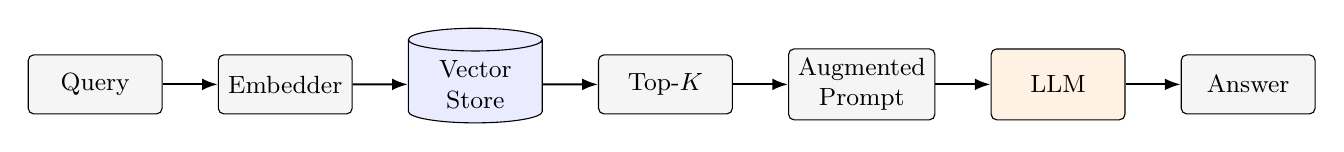
\begin{tikzpicture}[
  font=\small,
  node distance=0.55cm and 0.7cm,
  box/.style={draw, rounded corners=2pt, minimum width=1.7cm, minimum height=0.75cm, align=center, fill=VeryLightGray},
  store/.style={draw, cylinder, shape border rotate=90, aspect=0.25, minimum width=1.7cm, minimum height=1.0cm, align=center, fill=blue!8},
  llm/.style={draw, rounded corners=2pt, minimum width=1.7cm, minimum height=0.9cm, align=center, fill=orange!10},
  arr/.style={-{Latex[length=2mm]}, thick}
]
  \node[box] (q) {Query};
  \node[box, right=of q] (emb) {Embedder};
  \node[store, right=of emb] (db) {Vector\\Store};
  \node[box, right=of db] (top) {Top-$K$};
  \node[box, right=of top] (prompt) {Augmented\\Prompt};
  \node[llm, right=of prompt] (llm) {LLM};
  \node[box, right=of llm] (ans) {Answer};

  \draw[arr] (q) -- (emb);
  \draw[arr] (emb) -- (db);
  \draw[arr] (db) -- (top);
  \draw[arr] (top) -- (prompt);
  \draw[arr] (prompt) -- (llm);
  \draw[arr] (llm) -- (ans);
\end{tikzpicture}
\end{center}

\medskip
\begin{itemize}
\item Done \textbf{every time the user asks a question}.
\item Each query embeds once, retrieves a handful of chunks, and pays for only those tokens at the LLM stage.
\item \textbf{Ask-the-librarian analogy:} You walk up with a question, the librarian hands you 5 relevant pages, you read them and answer.
\item \textbf{Use the same embedder for indexing and querying} --- otherwise the geometry doesn't line up.
\end{itemize}
\end{frame}

%=============================================================================
\section{Chunking}
% PART IV: STEP 1 -- DOCUMENT INGESTION AND CHUNKING
%=============================================================================

\begin{frame}{Why Chunk At All?}
\begin{itemize}
\item Documents are too big to embed as a single vector. We must split them into smaller pieces --- \emph{chunks} --- before indexing.

\medskip
\item \textbf{Three reasons to chunk:}
\begin{enumerate}
    \item \textbf{Embedder input limits.} Most embedding models accept 512--8192 tokens per input. A 60-page FOMC transcript blows past every limit.
    \item \textbf{Granularity of relevance.} If you index a whole 30-page document as one vector, the embedding averages over many topics. A query about ``inflation expectations'' may match a document that contains \emph{one paragraph} on the topic --- but the average vector won't reflect it.
    \item \textbf{Generator context budget.} You only inject a few chunks into the LLM prompt. Smaller chunks $\Rightarrow$ more chunks fit $\Rightarrow$ richer evidence base.
\end{enumerate}

\medskip
\item \textbf{Trade-off:} Chunks too large $\Rightarrow$ noisy embeddings. Chunks too small $\Rightarrow$ context lost. \emph{Choosing chunk size is the most consequential decision in a RAG pipeline.}
\end{itemize}
\end{frame}

\begin{frame}{Chunking Strategies --- Overview}
\begin{center}
\renewcommand{\arraystretch}{1.35}
\begin{tabular}{|p{3.0cm}|p{5.0cm}|p{5.5cm}|}
\hline
\textbf{Strategy} & \textbf{How it splits} & \textbf{Trade-off} \\
\hline
Fixed-size & Every $N$ tokens & Simple; cuts mid-sentence \\
\hline
Recursive character & Hierarchy of separators (\textbackslash n\textbackslash n, \textbackslash n, \texttt{.}, space) & Respects structure; modern default \\
\hline
Sentence-window & One sentence per chunk + neighbors as context & High precision; many small chunks \\
\hline
Semantic & Cluster sentences by embedding similarity, split on cluster gaps & Topical coherence; expensive \\
\hline
Document-aware & Use doc structure (headings, sections, items) & Best with structured corpora; needs a parser \\
\hline
\end{tabular}
\end{center}

\bigskip
\textbf{Practical recommendation:} Start with \emph{recursive character} (LangChain default). Move to \emph{document-aware} when your corpus has rich structure (FOMC, 10-K, Congress). Use \emph{semantic} only after you have measured retrieval quality and can justify the cost.
\end{frame}

\begin{frame}{Fixed-Size vs.\ Recursive --- An Example}
\begin{itemize}
\item \textbf{Source paragraph} (FOMC minutes, simplified):
\begin{quote}
\small\itshape
``Participants observed that inflation remained elevated. Several noted that core services prices, especially shelter, continued to rise. A few participants expressed concern about persistence in wage growth. Most agreed that policy should remain restrictive.''
\end{quote}

\medskip
\item \textbf{Fixed 60-character chunks:}
\begin{quote}
\small\ttfamily
{[}``Participants observed that inflation remained elevat''] \\
{[}``ed. Several noted that core services prices, especi''] \\
{[}``ally shelter, continued to rise. A few participants''] \dots
\end{quote}
$\Rightarrow$ \textbf{Cuts mid-word.} Embeddings of these fragments are nearly useless.

\medskip
\item \textbf{Recursive chunking} (split on paragraph $\to$ sentence $\to$ word, target $\sim$120 chars):
\begin{quote}
\small\ttfamily
[``Participants observed that inflation remained elevated.''] \\
{[}``Several noted that core services prices, especially shelter, continued to rise.''] \\
{[}``A few participants expressed concern about persistence in wage growth.'']
\end{quote}
$\Rightarrow$ Each chunk is a self-contained sentence. Embeddings carry meaning.
\end{itemize}
\end{frame}

\begin{frame}{Semantic Chunking}
\begin{itemize}
\item \textbf{Idea:} Don't fix chunk size in advance. Instead, embed each sentence, measure similarity between adjacent sentences, and split where the similarity \emph{drops} --- i.e., where the topic changes.

\medskip
\item \textbf{Algorithm sketch:}
\begin{enumerate}
    \item Split the document into sentences.
    \item Embed each sentence with a fast embedder.
    \item Compute cosine similarity between consecutive sentence embeddings.
    \item Mark a chunk boundary wherever similarity falls below a threshold (or a percentile cutoff).
\end{enumerate}

\medskip
\item \textbf{Pros:} Each chunk is topically coherent --- you don't slice mid-thought.

\medskip
\item \textbf{Cons:} Costs an embedding pass over every sentence \emph{at indexing time}. For very large corpora this is non-trivial.

\medskip
\item \textbf{When to use:} When recursive chunking gives noisy retrieval and you have evidence that within-document topic shifts matter (long technical reports, multi-section speeches).
\end{itemize}
\end{frame}

\begin{frame}[fragile]{Practical Defaults + Code}
\begin{itemize}
\item \textbf{Sensible defaults} for institutional text:
\begin{itemize}
    \item Chunk size: 500--1000 tokens ($\sim$2--4 paragraphs)
    \item Chunk overlap: 10--20\% (so a sentence on a chunk boundary appears in both neighbors)
    \item \textbf{Always preserve metadata}: doc ID, page number, section heading, date, author
\end{itemize}

\medskip
\item \textbf{LangChain recursive chunker} (the de facto standard):
\begin{lstlisting}[language=Python]
from langchain.text_splitter import RecursiveCharacterTextSplitter

splitter = RecursiveCharacterTextSplitter(
    chunk_size=800,            # ~600 tokens
    chunk_overlap=100,         # ~80 tokens of overlap
    separators=["\n\n", "\n", ". ", " ", ""],
)

chunks = splitter.create_documents(
    texts=[fomc_minutes_text],
    metadatas=[{"meeting": "2024-06", "doc_type": "minutes"}],
)
\end{lstlisting}
\end{itemize}
\end{frame}

\begin{frame}{The Economist's Chunking Gotcha}
\begin{itemize}
\item Real institutional documents have \textbf{structure} that naive chunkers destroy.

\medskip
\item \textbf{FOMC minutes:} organized as \emph{speaker turns}. ``Participants generally agreed\dots'', ``A few members noted\dots''. Cutting across speaker boundaries fuses unrelated viewpoints.

\medskip
\item \textbf{Congressional Record:} hierarchical metadata --- Congress / session / chamber / date / speaker / bill. Lose the hierarchy and you can't filter or cite properly.

\medskip
\item \textbf{SEC 10-K filings:} standardized item numbers (Item 1, Item 1A Risk Factors, Item 7 MD\&A). A query about ``risk factors'' should retrieve only \emph{Item 1A} content --- which only works if you parse the structure first.

\medskip
\item \textbf{Practical fix:} Write a corpus-specific parser that emits chunks with rich metadata. Extra effort up front; massive payoff in retrieval quality and ability to filter.

\medskip
\item \textbf{Lesson:} Don't reach for the generic chunker. Let your corpus tell you what a chunk should be.
\end{itemize}
\end{frame}

%=============================================================================
\section{Embeddings}
% PART V: STEP 2 -- EMBEDDINGS
%=============================================================================

\begin{frame}{From Text to Vectors --- What and Why}
\begin{itemize}
\item An \textbf{embedding} is a function $E: \text{text} \to \mathbb{R}^d$ that maps a piece of text to a fixed-length vector of real numbers.

\medskip
\item Typical dimensionalities: $d \in \{384, 768, 1024, 1536, 3072\}$.

\medskip
\item \textbf{The crucial property:}
\[
\text{semantically similar texts } \;\Longrightarrow\; \text{nearby vectors in } \mathbb{R}^d
\]

\medskip
\item \textbf{Why this is useful:} Once your corpus lives in a vector space, ``find documents about inflation expectations'' becomes a \emph{geometric} operation: compute the embedding of the query, find its nearest neighbors among the document embeddings.

\medskip
\item \textbf{Recap from Lec.\ 7:} Embeddings appear \emph{inside} the transformer (token embeddings). Here we use the \emph{sentence-} or \emph{document-level} embedding produced by a separate retrieval-tuned model.
\end{itemize}
\end{frame}

\begin{frame}{Geometric Intuition}
\begin{center}
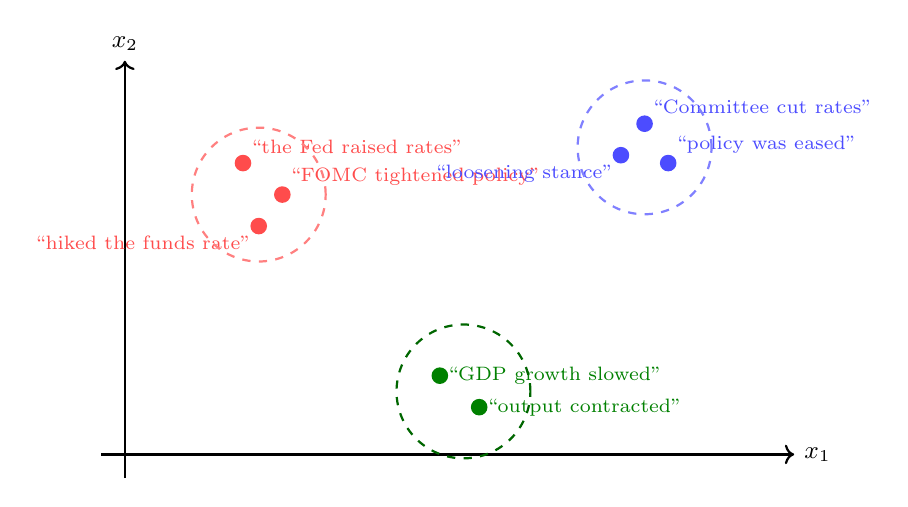
\begin{tikzpicture}[font=\small, scale=1.0]
  \draw[->, thick] (-0.3,0) -- (8.5,0) node[right] {$x_1$};
  \draw[->, thick] (0,-0.3) -- (0,5.0) node[above] {$x_2$};

  % Cluster A: hawkish / tightening
  \fill[red!70] (1.5,3.7) circle (3pt) node[above right, font=\scriptsize] {``the Fed raised rates''};
  \fill[red!70] (2.0,3.3) circle (3pt) node[above right, font=\scriptsize] {``FOMC tightened policy''};
  \fill[red!70] (1.7,2.9) circle (3pt) node[below left, font=\scriptsize] {``hiked the funds rate''};
  \draw[red!50, thick, dashed] (1.7,3.3) circle (0.85);

  % Cluster B: dovish / easing
  \fill[blue!70] (6.6,4.2) circle (3pt) node[above right, font=\scriptsize] {``Committee cut rates''};
  \fill[blue!70] (6.9,3.7) circle (3pt) node[above right, font=\scriptsize] {``policy was eased''};
  \fill[blue!70] (6.3,3.8) circle (3pt) node[below left, font=\scriptsize] {``loosening stance''};
  \draw[blue!50, thick, dashed] (6.6,3.9) circle (0.85);

  % Cluster C: unrelated
  \fill[green!50!black] (4.0,1.0) circle (3pt) node[right, font=\scriptsize] {``GDP growth slowed''};
  \fill[green!50!black] (4.5,0.6) circle (3pt) node[right, font=\scriptsize] {``output contracted''};
  \draw[green!40!black, thick, dashed] (4.3,0.8) circle (0.85);
\end{tikzpicture}
\end{center}

\textbf{Reading the picture:}
\begin{itemize}
\item Hawkish-tightening sentences cluster on the left.
\item Dovish-easing sentences cluster on the right.
\item Unrelated growth-related sentences sit elsewhere.
\item Distance in vector space $\approx$ semantic distance in meaning.
\end{itemize}

\textbf{This is the picture every RAG pipeline relies on.}
\end{frame}

\begin{frame}{Why This Works --- A Brief Lineage}
\begin{itemize}
\item \textbf{Word2Vec} (Mikolov et al., 2013): train a shallow network to predict context words. Word vectors emerge such that $\text{king} - \text{man} + \text{woman} \approx \text{queen}$. First convincing demonstration that vector geometry could capture meaning.

\medskip
\item \textbf{GloVe} (Pennington et al., 2014): factorize the global co-occurrence matrix. Same idea, different objective.

\medskip
\item \textbf{Sentence-BERT} (Reimers \& Gurevych, 2019): take a pretrained BERT, fine-tune it on \emph{sentence pairs} with a contrastive loss --- pulling paraphrases together, pushing unrelated sentences apart. Suddenly we can embed \emph{whole sentences}, not just words.

\medskip
\item \textbf{Modern retrieval embedders} (2023--2025): \texttt{bge-large-en}, \texttt{voyage-3}, OpenAI \texttt{text-embedding-3} --- transformer encoders trained on hundreds of millions of contrastive pairs from massive web-scale corpora.

\medskip
\item \textbf{Common thread:} Contrastive training pulls semantically related text together in vector space. The geometry is \emph{learned}, not designed.
\end{itemize}
\end{frame}

\begin{frame}{Modern Embedding Models --- Comparison}
\begin{center}
\renewcommand{\arraystretch}{1.25}
\small
\begin{tabular}{|l|c|c|l|l|}
\hline
\textbf{Model} & \textbf{Dim} & \textbf{Cost} & \textbf{Hosting} & \textbf{Notes} \\
\hline
OpenAI \texttt{text-embedding-3-small} & 1536 & \$0.02/M & API & cheap, fast, solid \\
\hline
OpenAI \texttt{text-embedding-3-large} & 3072 & \$0.13/M & API & top-tier accuracy \\
\hline
Cohere \texttt{embed-v3} & 1024 & \$0.10/M & API & strong on English \\
\hline
\texttt{voyage-3} & 1024 & \$0.12/M & API & top retrieval benchmarks \\
\hline
\texttt{all-MiniLM-L6-v2} & 384 & free & local & tiny, very fast, weaker \\
\hline
\texttt{bge-large-en-v1.5} & 1024 & free & local & top open-source \\
\hline
\texttt{e5-mistral-7b-instruct} & 4096 & free & local (GPU) & frontier open model \\
\hline
\end{tabular}
\end{center}

\bigskip
\textbf{For an academic researcher:}
\begin{itemize}
\item \textbf{Local + free:} \texttt{bge-large-en-v1.5}. Runs on a laptop GPU; competitive with paid APIs.
\item \textbf{Cloud + simple:} OpenAI \texttt{text-embedding-3-small}. Cheap, no infra.
\item \textbf{Top accuracy + budget:} \texttt{voyage-3} or OpenAI \texttt{3-large}.
\end{itemize}
\end{frame}

\begin{frame}{Economists' Embedding Example}
\begin{itemize}
\item \textbf{The setup.} Take every Federal Reserve Chair speech from 2010 to 2025 (Bernanke, Yellen, Powell). Embed each speech with \texttt{bge-large-en-v1.5}. Project to 2D with UMAP. Plot.

\medskip
\item \textbf{What you see:}
\begin{itemize}
    \item Crisis-era speeches (Bernanke 2010--2014) cluster together --- focused on QE, financial stability.
    \item Normalization-era speeches (Yellen 2015--2017) form a distinct cluster --- gradual exit, forward guidance.
    \item Pandemic and post-pandemic Powell (2020--2025) splits into two: 2020--2021 dovish ``patient'' speeches vs.\ 2022--2024 hawkish ``restrictive'' speeches.
\end{itemize}

\medskip
\item \textbf{Why this matters for research.} The clustering is generated \emph{purely from the text}, with no labels. The economist now has a reproducible measure of stance shifts that can be linked to interest-rate decisions, market reactions, or macro outcomes.

\medskip
\item \textbf{Real papers using this approach:}
\begin{itemize}
    \item Hansen, McMahon \& Prat (2018), \emph{QJE}: text analysis of FOMC transcripts.
    \item Shapiro \& Wilson (2021), \emph{Review of Economics and Statistics}: Fed sentiment from speeches.
    \item Gentzkow, Kelly \& Taddy (2019), \emph{JEL}: text as data, survey.
\end{itemize}
\end{itemize}
\end{frame}

\begin{frame}{The Domain-Adaptation Problem}
\begin{itemize}
\item Generic embedders are trained on the open web (Wikipedia, Common Crawl, books, code). They handle ordinary English well.

\medskip
\item \textbf{They struggle with economics jargon:}
\begin{itemize}
    \item ``\emph{patient}'' in a Fed statement = \emph{dovish} (a domain-specific code word).
    \item CUSIP codes, BEA NIPA tables, FRED series IDs --- alphanumeric strings with no semantic content for a generic embedder.
    \item Phrases like ``Section 13(3)'' or ``LSAP'' (Large-Scale Asset Purchases) are technical citations the model has never seen.
\end{itemize}

\medskip
\item \textbf{Two fixes:}
\begin{enumerate}
    \item \textbf{Fine-tune the embedder} on a domain corpus. Cheap (a few GPU-hours), big quality gains. Tools: \texttt{sentence-transformers} \texttt{MultipleNegativesRankingLoss}.
    \item \textbf{Hybrid retrieval} (Section VI). Combine dense embeddings with classical sparse retrieval (BM25), which catches exact-match queries the embedder misses.
\end{enumerate}

\medskip
\item \textbf{In practice:} Hybrid is usually cheaper and gets you 80\% of the gain. Reach for fine-tuning only when retrieval quality is your bottleneck.
\end{itemize}
\end{frame}

\begin{frame}[fragile]{Code: Embed FOMC Chunks}
\begin{lstlisting}[language=Python]
from sentence_transformers import SentenceTransformer

# 1. Load a strong open-source embedder
model = SentenceTransformer("BAAI/bge-large-en-v1.5")

# 2. Suppose `chunks` is a list of FOMC chunk strings
chunks = [
    "Participants observed that inflation remained elevated.",
    "Several noted that core services prices, especially shelter, continued to rise.",
    "Most agreed that policy should remain restrictive.",
    # ... thousands more
]

# 3. Embed -- one numpy vector per chunk
embeddings = model.encode(
    chunks,
    batch_size=32,
    normalize_embeddings=True,   # so cosine sim = dot product
    show_progress_bar=True,
)

print(embeddings.shape)
# (N_chunks, 1024) -- ready for the vector store
\end{lstlisting}
\end{frame}

%=============================================================================
\section{Vector Storage and Retrieval}
% PART VI: STEP 3 -- VECTOR STORAGE AND RETRIEVAL
%=============================================================================

\begin{frame}{Why a Vector Database?}
\begin{itemize}
\item Now we have millions of chunks, each with a 1024-dim embedding. \textbf{Where do they live?}

\medskip
\item \textbf{The naive option:} a flat numpy array on disk. Search by computing cosine similarity to every vector and sorting.
\begin{itemize}
    \item Works fine for $10{,}000$ vectors.
    \item At $1{,}000{,}000$ vectors a single query takes seconds.
    \item At $10{,}000{,}000$ it is impractical.
    \item No metadata filters. No incremental updates. No persistence.
\end{itemize}

\medskip
\item \textbf{A vector database} solves all four:
\begin{enumerate}
    \item \emph{Scale:} approximate nearest-neighbor (ANN) algorithms search millions of vectors in milliseconds.
    \item \emph{Metadata filters:} restrict search to ``date $\geq$ 2020 AND doc\_type = minutes.''
    \item \emph{Incremental updates:} add new chunks as new documents arrive, without rebuilding the index.
    \item \emph{Persistence:} the index lives on disk and survives process restarts.
\end{enumerate}
\end{itemize}
\end{frame}

\begin{frame}{Vector DB Landscape}
\begin{center}
\renewcommand{\arraystretch}{1.25}
\small
\begin{tabular}{|l|l|l|l|l|}
\hline
\textbf{System} & \textbf{Hosting} & \textbf{Scale} & \textbf{License} & \textbf{Best for} \\
\hline
FAISS (Meta) & local library & 100M+ & MIT & batch search, research \\
\hline
Chroma & local + server & 1M+ & Apache 2 & academic projects \\
\hline
Qdrant & local + cloud & 100M+ & Apache 2 & production-grade self-host \\
\hline
Weaviate & local + cloud & 100M+ & BSD & rich filtering, GraphQL \\
\hline
Milvus & distributed & 1B+ & Apache 2 & web-scale retrieval \\
\hline
Pinecone & managed cloud & 1B+ & proprietary & zero-ops, paid \\
\hline
pgvector & Postgres ext. & 10M+ & PostgreSQL & already on Postgres \\
\hline
\end{tabular}
\end{center}

\bigskip
\textbf{For an economist starting out:}
\begin{itemize}
\item \textbf{Chroma} or \textbf{FAISS} for laptop / cluster work. Free, local, simple.
\item \textbf{pgvector} if you already manage a Postgres database (e.g., institutional infrastructure).
\item \textbf{Pinecone / Qdrant cloud} if you need a hosted index and have budget.
\end{itemize}
\end{frame}

\begin{frame}{Similarity Search 101}
\begin{itemize}
\item Given a query vector $q$ and a database of vectors $\{d_1, d_2, \dots, d_N\}$, find the $K$ closest $d_i$ to $q$.

\medskip
\item \textbf{Three common similarity functions:}
\begin{itemize}
    \item \textbf{Cosine similarity:} $\;\cos(\theta) = \dfrac{q \cdot d_i}{\|q\| \, \|d_i\|}$
    \item \textbf{Dot product:} $\;q \cdot d_i$
    \item \textbf{(Negative) Euclidean distance:} $\;-\|q - d_i\|$
\end{itemize}

\medskip
\item \textbf{Why cosine is the default:} Cosine is invariant to vector magnitude. Modern embedders are typically L2-normalized at the end of the forward pass, in which case cosine $=$ dot product and both reduce to: \emph{higher dot product $\Rightarrow$ more similar}.

\medskip
\item \textbf{Geometric picture:} Each chunk is an arrow from the origin. The query is another arrow. Cosine similarity measures the angle between them. Two vectors pointing in the same direction (small angle) are deemed similar regardless of length.
\end{itemize}
\end{frame}

\begin{frame}{Approximate Nearest Neighbor (ANN)}
\begin{itemize}
\item \textbf{Exact search} computes similarity to \emph{every} vector in the database. Cost: $O(N \cdot d)$ per query.

\medskip
\item For $N = 10^7$ and $d = 1024$, that's $\sim$$10^{10}$ floating-point operations per query --- seconds of latency.

\medskip
\item \textbf{Approximate Nearest Neighbor:} Sacrifice a tiny bit of accuracy ($\sim$1\% recall loss) for orders-of-magnitude speedup.

\medskip
\item \textbf{Two dominant ANN families:}
\begin{itemize}
    \item \textbf{HNSW} (Hierarchical Navigable Small World): build a multi-layer graph of vectors; search by greedy walks on the graph. Default in Qdrant, Weaviate, pgvector.
    \item \textbf{IVF} (Inverted File): cluster vectors into Voronoi cells, search only the closest cells. Default in FAISS for very large indexes.
\end{itemize}

\medskip
\item \textbf{In practice} you won't choose the algorithm by hand --- you'll pick a vector DB and accept its default. But knowing the names helps when you read the docs.
\end{itemize}
\end{frame}

\begin{frame}{Hybrid Retrieval: Dense + Sparse}
\begin{itemize}
\item \textbf{The dense-only failure case:} A user asks ``find every speech mentioning \emph{Section 13(3)}.'' This is a precise legal-citation query.
\begin{itemize}
    \item Dense embeddings cluster similar \emph{meanings}, not similar \emph{strings}.
    \item ``Section 13(3)'' may not even be in the embedder's vocabulary.
    \item Result: top-10 neighbors are about the discount window in general --- not the specific section.
\end{itemize}

\medskip
\item \textbf{The fix:} also run a classical sparse retriever in parallel.
\begin{itemize}
    \item \textbf{BM25}: a TF-IDF-based ranking function that scores documents by exact term matches with the query.
    \item Catches everything dense retrieval misses on rare strings, acronyms, statute citations, ticker symbols, identifiers.
\end{itemize}

\medskip
\item \textbf{Combine the two via Reciprocal Rank Fusion (RRF):}
\[
\text{score}(d) = \sum_{r \in \{\text{dense, sparse}\}} \frac{1}{k + \text{rank}_r(d)}
\quad \text{(typically } k = 60 \text{)}
\]

\medskip
\item Hybrid retrieval is the \textbf{production default in 2025}. Pure dense is rarely competitive.
\end{itemize}
\end{frame}

\begin{frame}{Re-Ranking with Cross-Encoders}
\begin{itemize}
\item \textbf{Two-stage retrieval:}
\begin{enumerate}
    \item \textbf{First pass (bi-encoder):} fast, embeds query and documents \emph{independently}, returns top-50 candidates by cosine similarity.
    \item \textbf{Second pass (cross-encoder re-ranker):} slow, takes the query \emph{and} a candidate document \emph{together} as input, outputs a relevance score. Returns the top-5.
\end{enumerate}

\medskip
\item \textbf{Why this works.} A cross-encoder reads the query and document jointly --- so it can attend to which parts of the document actually answer the query. Bi-encoders cannot do this. The cost: cross-encoders are $\sim$100$\times$ slower per pair, so we only use them on the top-50 short-list.

\medskip
\item \textbf{Popular re-rankers:}
\begin{itemize}
    \item Cohere \texttt{Rerank} (paid API)
    \item \texttt{bge-reranker-large} (free, local)
    \item \texttt{ms-marco-MiniLM-L-12-v2} (free, smaller)
\end{itemize}

\medskip
\item \textbf{Why re-ranking matters in practice.} The top-1 hit from a bi-encoder is often outranked by something the re-ranker catches. Without re-ranking you ask the LLM the wrong question.
\end{itemize}
\end{frame}

\begin{frame}{Metadata Filters}
\begin{itemize}
\item Pure semantic search is insufficient when the query has \emph{structural} constraints.

\medskip
\item \textbf{Real example:} \emph{``Find all FOMC discussions of unemployment from 2020 onwards, excluding press conferences.''}
\begin{itemize}
    \item ``Discussions of unemployment'' $\Rightarrow$ semantic search.
    \item ``From 2020 onwards'' $\Rightarrow$ filter on \texttt{date $\geq$ 2020-01-01}.
    \item ``Excluding press conferences'' $\Rightarrow$ filter on \texttt{doc\_type $\neq$ press\_conference}.
\end{itemize}

\medskip
\item Modern vector DBs let you combine vector similarity with SQL-style metadata filters in a single query.

\medskip
\item \textbf{This is exactly why preserving rich metadata at chunking time matters} (Section IV gotcha). If your chunks don't carry \texttt{date}, \texttt{doc\_type}, \texttt{speaker}, etc., you cannot filter on them later.

\medskip
\item \textbf{Rule of thumb:} Add \emph{more} metadata than you think you need. It is cheap at index time and impossible to reconstruct after the fact.
\end{itemize}
\end{frame}

\begin{frame}[fragile]{Code: Build a Chroma Index and Query It}
\begin{lstlisting}[language=Python]
import chromadb
from sentence_transformers import SentenceTransformer

model = SentenceTransformer("BAAI/bge-large-en-v1.5")

# 1. Persistent Chroma client (data lives on disk)
client = chromadb.PersistentClient(path="./fomc_index")
coll = client.get_or_create_collection("fomc")

# 2. Add chunks with metadata
coll.add(
    ids=[f"chunk_{i}" for i in range(len(chunks))],
    documents=chunks,
    embeddings=model.encode(chunks, normalize_embeddings=True).tolist(),
    metadatas=[{"meeting": "2024-06", "doc_type": "minutes"} for _ in chunks],
)

# 3. Query: "How did the Committee discuss inflation expectations?"
query = "How did the Committee discuss inflation expectations?"
q_emb = model.encode([query], normalize_embeddings=True).tolist()

results = coll.query(
    query_embeddings=q_emb,
    n_results=5,
    where={"doc_type": "minutes"},   # metadata filter
)

for doc, meta in zip(results["documents"][0], results["metadatas"][0]):
    print(meta["meeting"], "->", doc[:80])
\end{lstlisting}
\end{frame}

%=============================================================================
\section{Beyond Dense Retrieval}
% PART VII: GRAPH-BASED AND HIERARCHICAL RAG
%=============================================================================

\begin{frame}{Where Vanilla Vector RAG Starts to Break}
\begin{itemize}
\item Dense retrieval is a \textbf{local similarity machine}. It finds chunks whose wording or meaning is close to the query.

\medskip
\item That is enough for many lookup questions, but it misses three important structures:
\begin{enumerate}
    \item \textbf{Relationships between objects.} Two chunks may matter because their entities are linked, even if the wording differs.
    \item \textbf{Global structure.} Nearest-neighbor search has no notion of discourse communities, themes, or argument clusters across an entire corpus.
    \item \textbf{Coverage.} If the same fact appears in many chunks, top-$K$ retrieval often returns duplicates instead of a representative overview.
\end{enumerate}

\medskip
\item \textbf{Economist examples:}
\begin{itemize}
    \item ``Which Senators most often connect inflation to housing supply constraints?''
    \item ``What are the main camps in recent papers on LLMs and education?''
\end{itemize}

\medskip
\item Once the question is \textbf{multi-hop} or \textbf{corpus-level}, plain top-$K$ chunk retrieval is often the wrong abstraction.
\end{itemize}
\end{frame}

\begin{frame}{Knowledge Graphs: Adding Structure to Retrieval}
\begin{columns}[T,totalwidth=\textwidth]
\column{0.50\textwidth}
\begin{itemize}
\item A \textbf{knowledge graph (KG)} stores facts as \textbf{nodes + edges} rather than isolated chunks.

\medskip
\item Canonical representation: \texttt{<head, relation, tail>}, e.g.\
\texttt{<Powell, discusses, inflation expectations>}.

\medskip
\item In graph-based RAG, the index can mix \textbf{entity nodes}, \textbf{chunk nodes}, and \textbf{community summaries}.

\medskip
\item The gain is simple: retrieval is no longer ``find text that sounds similar.'' It becomes ``find the \emph{relevant subgraph}.'' 
\end{itemize}

\column{0.46\textwidth}
\centering

\includegraphics[width=\linewidth]{graph_rag_share/knowledge_graph_example.png}

\scriptsize
Once facts are stored as a graph, retrieval can follow links rather than isolated paragraphs.
\end{columns}
\end{frame}

\begin{frame}{Graph-Based RAG: Offline vs.\ Online}
\begin{columns}[T,totalwidth=\textwidth]
\column{0.34\textwidth}
\small
\textbf{Offline indexing}
\begin{itemize}
    \item chunk the corpus
    \item extract entities and relations
    \item build the graph and any auxiliary indexes
    \item optionally detect communities and summarize them
\end{itemize}

\textbf{Online querying}
\begin{itemize}
    \item interpret or rewrite the question
    \item retrieve nodes, edges, chunks, or communities
    \item expand to a relevant subgraph
    \item build the prompt and ask the LLM to answer
\end{itemize}

\column{0.62\textwidth}
\centering

\includegraphics[width=\linewidth]{graph_rag_share/graphrag_pipeline.png}

\scriptsize
GraphRAG-style intuition: communities are built offline, then query-focused summaries are composed online.
\end{columns}
\end{frame}

\begin{frame}{Choosing the Retrieval Architecture}
\begin{center}
\renewcommand{\arraystretch}{1.25}
\small
\begin{tabular}{|p{3.2cm}|p{3.1cm}|p{5.8cm}|}
\hline
\textbf{Question type} & \textbf{Best first choice} & \textbf{Why} \\
\hline
Precise factual lookup or citation hunt & Hybrid dense + sparse RAG & Exact strings, dates, and citations matter more than global structure. \\
\hline
Specific multi-hop entity question & Graph-based RAG & The answer depends on linked entities, paths, or neighborhoods rather than one chunk. \\
\hline
Broad abstract summarization over a large corpus & GraphRAG / RAPTOR-style hierarchy & You need coverage of themes or communities, not just the closest paragraphs. \\
\hline
Fast prototype on a changing corpus & Vanilla RAG first & A flat vector index is easy to build and update; add graph structure only if it buys real accuracy. \\
\hline
\end{tabular}
\end{center}

\bigskip
\textbf{Rule of thumb:} start with hybrid dense+sparse RAG. Escalate to graph or hierarchical retrieval when the task requires \emph{relationships}, \emph{coverage}, or \emph{multi-hop reasoning}.
\end{frame}

\begin{frame}{Representative Systems You Should Recognize}
\begin{center}
\renewcommand{\arraystretch}{1.2}
\scriptsize
\begin{tabular}{|p{2.0cm}|p{3.2cm}|p{2.7cm}|p{4.2cm}|}
\hline
\textbf{System} & \textbf{Core idea} & \textbf{Best at} & \textbf{What to remember} \\
\hline
Microsoft GraphRAG & Build a KG, detect communities, summarize them, then retrieve by community plus local evidence & Query-focused summarization & Strong when the user asks for an overview of a large corpus rather than one citation. \\
\hline
LightRAG & Dual-level retrieval: local entity-level evidence plus high-level thematic evidence & Mixed local/global questions & A pragmatic design that tries to keep graph retrieval lightweight. \\
\hline
HippoRAG & Expand a memory graph with KNN links, then run personalized PageRank from the query & Multi-hop recall & Explicitly treats retrieval as traversing associative memory. \\
\hline
RAPTOR & Recursively cluster chunks and summarize the clusters into a tree & Long-document and abstract QA & Not a full KG, but the same core idea: retrieve from higher-level structure when chunks alone are too local. \\
\hline
\end{tabular}
\end{center}

\medskip
\footnotesize
Key references: Edge et al.\ (2024), Guo et al.\ (2024), Gutierrez et al.\ (2024), and Sarthi et al.\ (2024).
\end{frame}

\begin{frame}{Visual Snapshots: GraphRAG and LightRAG}
\begin{columns}[T,totalwidth=\textwidth]
\column{0.49\textwidth}
\textbf{GraphRAG}


\includegraphics[width=0.96\linewidth]{graph_rag_share/graphrag_pipeline.png}

\scriptsize Community summaries provide global coverage for abstract questions.

\column{0.49\textwidth}
\textbf{LightRAG}


\includegraphics[width=\linewidth]{graph_rag_share/lightrag_workflow.png}

\scriptsize Dual-level retrieval: local entities plus higher-level themes.
\end{columns}
\end{frame}

\begin{frame}{Visual Snapshots: HippoRAG and RAPTOR}
\begin{columns}[T,totalwidth=\textwidth]
\column{0.49\textwidth}
\textbf{HippoRAG}


\includegraphics[width=\linewidth]{graph_rag_share/hipporag_workflow.png}

\scriptsize Personalized PageRank expands a memory-like graph neighborhood.

\column{0.49\textwidth}
\textbf{RAPTOR}


\includegraphics[width=\linewidth]{graph_rag_share/raptor_tree.png}

\scriptsize Recursive clustering and summarization into a tree.
\end{columns}
\end{frame}

\begin{frame}{What Recent Graph-RAG Benchmarks Suggest}
\begin{columns}[T,totalwidth=\textwidth]
\column{0.40\textwidth}
\small
\begin{itemize}
\item \textbf{Chunk quality still dominates.} Better chunks help almost every architecture.

\medskip
\item \textbf{High-level structure helps abstract questions.} Community reports and hierarchies beat a bag of similar chunks when the user wants synthesis.

\medskip
\item \textbf{Specific QA can still need structure.} Hard factual questions often require linking several local pieces of evidence.

\medskip
\item \textbf{Graph maintenance is expensive.} Build cost, token cost, and dynamic updates remain real bottlenecks.
\end{itemize}

\column{0.56\textwidth}
\centering

\includegraphics[width=\linewidth]{graph_rag_share/benchmark_efficiency.png}

\scriptsize
Illustrative benchmark from the donor deck: graph-RAG variants can buy capability, but often at sharply different token and latency costs.
\end{columns}
\end{frame}

%=============================================================================
\section{Augmented Generation}
% PART VIII: STEP 4 -- AUGMENTED GENERATION
%=============================================================================

\begin{frame}{From Retrieved Chunks to a Final Answer}
\begin{itemize}
\item We now have the top-$K$ chunks for the user's query (typically $K = 3$ to $10$). What do we do with them?

\medskip
\item \textbf{Insert them into a prompt template, send to the LLM.} The model sees:
\begin{enumerate}
    \item System instructions (how to behave)
    \item The retrieved chunks (the evidence)
    \item The user question
    \item Output-format instructions (how to cite)
\end{enumerate}

\medskip
\item The LLM now \textbf{generates} an answer that is \emph{grounded in the retrieved evidence}.

\medskip
\item This is the only place a generative model is used in the whole pipeline. Everything before this --- chunking, embedding, retrieval --- exists to put high-quality evidence in front of the model.

\medskip
\item \textbf{The single most important design choice} at this stage: the \emph{prompt template}.
\end{itemize}
\end{frame}

\begin{frame}[fragile]{Prompt Template --- Anatomy}
A real RAG prompt has four parts. Lines below are color-coded by role:
\begin{lstlisting}
SYSTEM:
You are a research assistant for academic economists.
Answer the user's question using ONLY the context below.
If the context does not contain the answer, reply
exactly: "I don't know based on the provided sources."
Cite sources inline using [doc_id:page] notation.

CONTEXT:
[1] (fomc_2024_06:p3)
"Participants observed that inflation remained elevated..."

[2] (fomc_2024_06:p4)
"Several noted that core services prices, especially shelter,
continued to rise..."

[3] (powell_2024_press:p2)
"The Committee remains attentive to the risks that inflation poses..."

QUESTION:
How did the FOMC discuss inflation expectations in June 2024?

INSTRUCTIONS:
Answer in 2-3 sentences. Cite each claim inline as [doc_id:page].
\end{lstlisting}
\end{frame}

\begin{frame}{Source Attribution Mechanics}
\begin{itemize}
\item \textbf{Why economists need this:} Every claim in an academic paper must be \emph{traceable to a source}. An ungrounded LLM output is not citable. A grounded output is.

\medskip
\item \textbf{How to enforce:}
\begin{enumerate}
    \item At chunking time, give every chunk a stable \texttt{doc\_id} and \texttt{page} (or \texttt{turn}, or \texttt{section}).
    \item At retrieval time, return the metadata along with the chunk text.
    \item In the prompt template, label each chunk \texttt{[1] (doc\_id:page)} and instruct the model to cite using that label.
    \item In post-processing, replace the model's inline citations with hyperlinks back to the original document.
\end{enumerate}

\medskip
\item \textbf{Before / after example:}
\begin{itemize}
    \item \emph{Ungrounded:} ``The FOMC was concerned about inflation persistence in 2024.''
    \item \emph{Grounded:} ``The FOMC was concerned about inflation persistence in mid-2024 \texttt{[fomc\_2024\_06:p3]}, particularly in core services prices including shelter \texttt{[fomc\_2024\_06:p4]}.''
\end{itemize}
\end{itemize}
\end{frame}

\begin{frame}{Refusal and Faithfulness}
\begin{itemize}
\item \textbf{``I don't know'' is a feature, not a bug.}

\medskip
\item In an academic context, \emph{fabricating an answer is far worse than refusing to answer.}

\medskip
\item \textbf{Faithfulness} (the answer is fully supported by the retrieved context) matters more than \emph{fluency} (the answer reads well). A fluent fabrication is the worst possible outcome for research.

\medskip
\item \textbf{How to enforce refusal:}
\begin{itemize}
    \item Explicit instruction in the system prompt: ``If the context does not contain the answer, reply exactly: I don't know based on the provided sources.''
    \item Set generation \texttt{temperature} low (e.g.\ 0.0--0.2) to discourage creative inference.
    \item In post-processing, run a faithfulness check (Section X) and flag answers whose claims aren't supported by retrieved chunks.
\end{itemize}

\medskip
\item \textbf{Example refusal (good behavior):}
\begin{quote}
\small\itshape
``I don't know based on the provided sources. The retrieved minutes from June 2024 do not discuss the impact of fiscal policy.''
\end{quote}

\medskip
\item This protects the researcher from quoting fiction.
\end{itemize}
\end{frame}

\begin{frame}{Worked Example: Full Pipeline Run}
\textbf{Query.} \emph{``How did Powell discuss inflation expectations in 2023 press conferences?''}

\medskip
\textbf{Pipeline trace:}
\begin{enumerate}
\item \textbf{Embed query} with \texttt{bge-large-en-v1.5} $\to$ 1024-d vector.
\medskip
\item \textbf{Retrieve top-50} via Chroma + BM25 hybrid. Filter: \texttt{doc\_type = press\_conference} AND \texttt{year = 2023}.
\medskip
\item \textbf{Re-rank} the 50 with \texttt{bge-reranker-large} $\to$ top-5.
\medskip
\item \textbf{Inject top-5 chunks} into the prompt template (previous slide), tagged \texttt{[powell\_2023\_03:p4]}, \texttt{[powell\_2023\_06:p2]}, \dots
\medskip
\item \textbf{Send to GPT-4o} at \texttt{temperature=0.1}. Receives:
\begin{quote}
\small\itshape
``In 2023 press conferences, Chair Powell repeatedly emphasized that long-run inflation expectations remained well anchored \texttt{[powell\_2023\_03:p4]}, while noting that short-run expectations had risen with realized inflation \texttt{[powell\_2023\_06:p2]}. By the end of the year, he highlighted that survey- and market-based measures had begun to ease \texttt{[powell\_2023\_12:p3]}.''
\end{quote}
\medskip
\item \textbf{Post-process:} convert inline citations to clickable links back to the original transcript pages.
\end{enumerate}
\end{frame}

%=============================================================================
\section{RAG vs Fine-Tuning}
% PART VIII: RAG VS FINE-TUNING
%=============================================================================

\begin{frame}{Decision Matrix: RAG vs.\ Fine-Tuning}
\begin{center}
\renewcommand{\arraystretch}{1.3}
\small
\begin{tabular}{|p{4.6cm}|c|c|}
\hline
\textbf{Dimension} & \textbf{RAG} & \textbf{Fine-tuning} \\
\hline
Knowledge freshness (update daily) & \checkmark\checkmark & \texttimes \\
\hline
Source attribution / citations & \checkmark\checkmark & \texttimes \\
\hline
Reduces hallucination & \checkmark\checkmark & limited \\
\hline
Cost to add new documents & near zero & re-train \\
\hline
Latency at query time & moderate & low \\
\hline
Style adaptation (e.g.\ ``write like the Fed'') & \texttimes & \checkmark\checkmark \\
\hline
Output-format adaptation (structured JSON) & limited & \checkmark\checkmark \\
\hline
\end{tabular}
\end{center}

\bigskip
\textbf{Reading the table:} RAG dominates on the four dimensions that matter most for research --- freshness, attribution, hallucination control, and update cost. Fine-tuning dominates on style and format, which matter for production deployments but rarely for research.
\end{frame}

\begin{frame}{When Fine-Tuning Still Makes Sense}
\begin{itemize}
\item \textbf{Style transfer.} You want the model to \emph{write like a Federal Reserve economist} --- the cadence, the hedging, the preferred phrasing. Hand the model a thousand examples of FOMC minutes and fine-tune. RAG can't teach style.

\medskip
\item \textbf{Structured-output formatting.} You want the model to always emit a JSON dictionary of DSGE parameters. Fine-tune on $\sim$500 input/output pairs. Cheaper than prompt-engineering an enforced schema.

\medskip
\item \textbf{Specialized vocabulary.} The model needs to recognize that \texttt{LSAP} = Large-Scale Asset Purchase or that \texttt{NIPA} = National Income and Product Accounts. Some tokens may not even be in the base tokenizer; fine-tuning can teach the model to handle them gracefully.

\medskip
\item \textbf{Latency-critical settings.} Fine-tuned models embed knowledge in weights, so they don't need a retrieval round-trip. Useful for real-time applications --- but rarely a binding constraint for research.

\medskip
\item \textbf{Crucial caveat:} Fine-tuning $\neq$ teaching new \emph{facts}. Models often memorize facts unreliably during fine-tuning and still hallucinate. \emph{If you want the model to know new facts, use RAG.}
\end{itemize}
\end{frame}

\begin{frame}{The Hybrid Pattern}
\begin{itemize}
\item In production, the modern pattern is \textbf{both, in different roles}:

\medskip
\item \textbf{Fine-tune the embedding model} on a domain corpus (say, 100K FOMC sentences with synthetic query-document pairs). This is \emph{cheap} ($\sim$\$50 of compute) and improves retrieval quality dramatically.

\medskip
\item \textbf{Use a general-purpose LLM as the generator} (Claude, GPT-4o). No fine-tuning of the big model.

\medskip
\item \textbf{Use RAG as the glue.} The fine-tuned embedder ensures that the retriever finds the right chunks; the general LLM ensures fluent, faithful generation.

\medskip
\item \textbf{Why this works.} You get domain understanding (from fine-tuning) and freshness + attribution (from RAG), without the cost or fragility of fine-tuning a 70B-parameter generator.

\medskip
\item This is the dominant production architecture in 2025 for any LLM application that touches a specialized corpus --- legal, medical, financial, academic.
\end{itemize}
\end{frame}

\begin{frame}{Cost \& Operational Comparison}
\begin{center}
\renewcommand{\arraystretch}{1.35}
\small
\begin{tabular}{|p{4.0cm}|p{4.2cm}|p{4.5cm}|}
\hline
& \textbf{Fine-tuning a 7B model} & \textbf{RAG with general LLM} \\
\hline
Setup cost & $\sim$\$500 + 12 GPU-hours & $\sim$\$50 (embedding pass + Chroma) \\
\hline
Time to first answer & 2--3 days (data prep + train) & 1 afternoon \\
\hline
Cost per query & low (model is local) & API call: \$0.001--\$0.05 \\
\hline
Update with new docs & re-train weekly & add chunks in seconds \\
\hline
Source citations & no & yes \\
\hline
Skill needed & ML engineer & researcher with Python \\
\hline
\end{tabular}
\end{center}

\bigskip
\textbf{For a typical academic project} --- a few thousand queries against a curated corpus --- RAG is 10$\times$ to 100$\times$ cheaper end-to-end and gives \emph{better} answers. Fine-tuning is the right tool only when you genuinely need style or format control.
\end{frame}

%=============================================================================
\section{Economic Applications}
% PART IX: APPLICATIONS IN ECONOMIC RESEARCH
%=============================================================================

\begin{frame}{Use Case 1: FOMC Minutes \& Press Conferences}
\begin{itemize}
\item \textbf{Corpus.} The Federal Reserve publishes statements (post-meeting), minutes (3-week lag), press conference transcripts, and (5-year lag) full meeting transcripts. Available 1993--present at \texttt{federalreserve.gov}.

\medskip
\item \textbf{Index pipeline:}
\begin{enumerate}
    \item Scrape PDFs / HTML from the Fed archive.
    \item Parse into speaker turns (minutes) or Q\&A pairs (press conferences).
    \item Chunk with rich metadata: \texttt{meeting\_date}, \texttt{doc\_type}, \texttt{speaker}, \texttt{topic\_section}.
    \item Embed with \texttt{bge-large-en-v1.5}.
    \item Store in Chroma; run BM25 in parallel for hybrid retrieval.
\end{enumerate}

\medskip
\item \textbf{Example research queries:}
\begin{itemize}
    \item \emph{``How did the Committee's framing of inflation expectations evolve from 2021 to 2024?''}
    \item \emph{``Find every appearance of `transitory' in FOMC minutes between 2020 and 2022.''}
    \item \emph{``Which participants most often dissented on rate decisions, 2017--2024?''}
\end{itemize}

\medskip
\item \textbf{Reference:} Hansen, McMahon \& Prat (2018), \emph{QJE}, ``Transparency and Deliberation Within the FOMC: A Computational Linguistics Approach.''
\end{itemize}
\end{frame}

\begin{frame}{Use Case 2: NBER Working Papers}
\begin{itemize}
\item \textbf{Corpus.} $\sim$32{,}000 NBER working papers, 1973--present, available at \texttt{nber.org}. Each has metadata: title, abstract, authors, JEL codes, full PDF.

\medskip
\item \textbf{Use case: literature review automation.} Instead of typing keywords into Google Scholar and reading 50 abstracts, ask:
\begin{quote}
\small\itshape
``Find all NBER working papers from 2019 onwards that estimate the slope of the Phillips curve. Return title, authors, year, the central estimate, and the data source.''
\end{quote}

\medskip
\item \textbf{Pipeline:}
\begin{enumerate}
    \item Index titles + abstracts as one collection (cheap, fast, good for keyword screening).
    \item Index full-paper chunks as a second collection (richer evidence for follow-up questions).
    \item Hybrid retrieval over both. Filter on \texttt{year}, \texttt{JEL\_code}, \texttt{author}.
    \item Generator outputs a structured table from retrieved papers.
\end{enumerate}

\medskip
\item \textbf{Caveat:} Always verify citations against the actual NBER record. Even with RAG, models occasionally garble author lists or year fields.

\medskip
\item \textbf{This is one of the highest-value RAG applications for an active researcher.}
\end{itemize}
\end{frame}

\begin{frame}{Use Case 3: Congressional Record \& Legislative Text}
\begin{itemize}
\item \textbf{Corpus.} The Congressional Record contains every speech delivered on the House and Senate floors since 1873. Daily editions are available at \texttt{congress.gov}.

\medskip
\item \textbf{Use case: tracking how policy debates frame economic issues over time.}
\begin{itemize}
    \item ``How has the rhetoric around `inflation' shifted in House Banking Committee testimony from 2008 to 2024?''
    \item ``Which Senators most frequently cite Federal Reserve research in floor speeches?''
\end{itemize}

\medskip
\item \textbf{The structural challenge.} Congressional Record has a deep hierarchy --- Congress / session / chamber / date / speaker / bill / section. The Section IV chunking gotcha applies in full force. A naive chunker that ignores this hierarchy will produce essentially un-citable retrieval results.

\medskip
\item \textbf{Practical fix:} Use a Congress-specific parser (e.g.\ \texttt{congress-api-python}) to extract clean speaker turns with all metadata, then feed those into the chunker.

\medskip
\item \textbf{Reference:} Gentzkow, Shapiro \& Taddy (2019), \emph{Econometrica}, ``Measuring Group Differences in High-Dimensional Choices: Method and Application to Congressional Speech.''
\end{itemize}
\end{frame}

\begin{frame}{Use Case 4: SEC 10-K Filings (Item 1A Risk Factors)}
\begin{itemize}
\item \textbf{Corpus.} EDGAR hosts $\sim$5{,}000{,}000 SEC filings, including the annual 10-K reports of every public US firm. Each 10-K has a standardized ``Item 1A: Risk Factors'' section disclosing material risks.

\medskip
\item \textbf{Use case: cross-firm comparison of disclosed risks.}
\begin{itemize}
    \item \emph{``Compare how the four largest US banks discussed interest-rate risk in their 2022 vs.\ 2023 10-K filings.''}
    \item \emph{``Find all 10-K filings from energy firms in 2024 that mention transition risk from climate policy.''}
\end{itemize}

\medskip
\item \textbf{Pipeline:}
\begin{enumerate}
    \item Use \texttt{sec-edgar-downloader} to pull 10-Ks.
    \item Run a section-aware parser to extract Item 1A only.
    \item Chunk \emph{within} Item 1A, preserving \texttt{cik}, \texttt{ticker}, \texttt{filing\_date}, \texttt{fiscal\_year}.
    \item Store in Chroma. Hybrid retrieval with metadata filter on \texttt{ticker} for cross-firm queries.
\end{enumerate}

\medskip
\item \textbf{Reference:} Loughran \& McDonald (2011), \emph{JF}, ``When Is a Liability Not a Liability? Textual Analysis, Dictionaries, and 10-Ks.'' Lopez-Lira (2023), ``Risk Factors That Matter.''
\end{itemize}
\end{frame}

\begin{frame}{Use Case 5: Cross-Country Central Bank Speeches}
\begin{itemize}
\item \textbf{Corpus.} The Bank for International Settlements maintains a unified archive of central bank speeches from $\sim$60 institutions, 1997--present, at \texttt{bis.org/cbspeeches}. Other primary sources: ECB, BoE, BoJ, RBA, BoC, RBI, PBoC.

\medskip
\item \textbf{Use case: comparative monetary policy analysis.}
\begin{itemize}
    \item \emph{``How did major central banks frame the post-COVID inflation surge in 2022 speeches? Compare the Fed, ECB, BoE, and BoJ.''}
    \item \emph{``Which central banks most often cite financial-stability concerns alongside inflation, 2010--2024?''}
\end{itemize}

\medskip
\item \textbf{Pipeline notes:}
\begin{itemize}
    \item Add \texttt{country}, \texttt{institution}, \texttt{speaker\_role}, \texttt{language} as metadata.
    \item For non-English speeches, either use a multilingual embedder (\texttt{multilingual-e5-large}) or translate first.
    \item Hybrid retrieval is critical --- many speeches use country-specific institutional jargon a generic embedder won't recognize.
\end{itemize}

\medskip
\item \textbf{This use case is essentially impossible without RAG --- no human can read $\sim$10{,}000 speeches across $\sim$60 institutions per year.}
\end{itemize}
\end{frame}

\begin{frame}{Use Case 6: Combining Structured + Unstructured}
\begin{itemize}
\item RAG isn't only for unstructured text. The most powerful pattern combines a \textbf{structured database} (e.g.\ FRED time series, BEA NIPA tables) with an \textbf{unstructured text store} (Fed speeches, FOMC minutes).

\medskip
\item \textbf{Example query:}
\begin{quote}
\small\itshape
``In months when the unemployment rate fell below 4\%, what did the Fed publicly say about labor markets?''
\end{quote}

\medskip
\item \textbf{Pipeline:}
\begin{enumerate}
    \item \emph{Structured side:} SQL on FRED data. \texttt{SELECT date FROM unrate WHERE value < 4.0;}
    \item \emph{Unstructured side:} retrieve speeches and FOMC minutes whose \texttt{date} falls within those months.
    \item Pass the joined evidence to the LLM with a prompt that says ``summarize how Fed officials characterized the labor market in these specific months.''
\end{enumerate}

\medskip
\item \textbf{This pattern} --- structured SQL filter $\to$ semantic retrieval $\to$ generation --- is uniquely useful for empirical economists. It bridges what economists already know how to do (data) with what they couldn't do before (text at scale).
\end{itemize}
\end{frame}

\begin{frame}{Synthesis: Three Workflow Patterns}
\begin{enumerate}
\item \textbf{Literature review.} Index a paper repository (NBER, SSRN, RePEc). Query: ``find work on X, summarize, return citations.'' Saves days per project.

\medskip
\item \textbf{Policy-text monitoring over time.} Index an institutional corpus (FOMC, Congress, central banks). Query: ``how did the framing of Y evolve from year A to year B?'' Turns institutional text into a longitudinal research instrument.

\medskip
\item \textbf{Cross-sectional comparative analysis.} Index a corpus where the unit of analysis is a firm or country (10-Ks, central bank speeches). Query: ``compare how entity-1, entity-2, \dots\ discussed Z in year Y.'' Enables cross-firm and cross-country comparisons that were previously infeasible at scale.
\end{enumerate}

\bigskip
\textbf{Methodological punchline.} RAG turns institutional text from \emph{background reading} into a \emph{queryable research instrument}. That is the new capability. Everything else --- chunking, embeddings, vector stores --- is plumbing.
\end{frame}

%=============================================================================
\section{Failure Modes and Evaluation}
% PART X: LIMITATIONS, EVALUATION, AND FAILURE MODES
%=============================================================================

\begin{frame}{When RAG Fails}
\textbf{Six common failure modes:}
\begin{enumerate}
\item \textbf{Retriever miss.} Relevant document exists but the embedder ranks it outside top-$K$. Often caused by terminology mismatch.

\medskip
\item \textbf{Re-ranker promotes the wrong context.} Cross-encoder mis-scores; the LLM gets a confident-but-irrelevant chunk.

\medskip
\item \textbf{Generator ignores the retrieved context.} The LLM falls back on its parametric memory and answers from training data --- often confidently and incorrectly.

\medskip
\item \textbf{Chunk boundary cuts critical information.} The fact spans the boundary between two chunks; neither chunk alone contains the answer.

\medskip
\item \textbf{Outdated index.} The corpus has been updated, but the index hasn't been re-run. The retriever returns stale chunks.

\medskip
\item \textbf{Ambiguous query.} ``Inflation'' could mean CPI, PCE, expectations, or asset prices. The retriever picks one interpretation; the user wanted another.
\end{enumerate}
\end{frame}

\begin{frame}{Mitigations --- One per Failure Mode}
\begin{itemize}
\item \textbf{Retriever miss} $\Rightarrow$ \emph{query expansion} and \emph{HyDE} (hypothetical document embeddings: ask the LLM to draft a fake answer, embed \emph{that}, retrieve nearest documents). Also: hybrid sparse + dense retrieval.

\medskip
\item \textbf{Re-ranker mis-scores} $\Rightarrow$ try a stronger re-ranker (\texttt{bge-reranker-v2}); train a domain-specific re-ranker on labeled query-document pairs.

\medskip
\item \textbf{Generator ignores context} $\Rightarrow$ stricter system prompt (``Answer ONLY from the context''); lower temperature; faithfulness check in post-processing.

\medskip
\item \textbf{Chunk boundary cuts information} $\Rightarrow$ semantic chunking; larger chunk overlap; or use a parent-document retriever (retrieve a chunk, return its parent paragraph).

\medskip
\item \textbf{Outdated index} $\Rightarrow$ incremental ingestion pipeline triggered when source documents change; nightly re-embed for high-churn corpora.

\medskip
\item \textbf{Ambiguous query} $\Rightarrow$ query rewriting (ask the LLM to clarify or expand the query before retrieval); multi-query retrieval (generate $N$ paraphrases, retrieve for each, fuse).
\end{itemize}
\end{frame}

\begin{frame}{Evaluation: The RAGAS Framework}
\begin{itemize}
\item Es, James, Espinosa-Anke \& Schockaert (2023), ``RAGAS: Automated Evaluation of Retrieval Augmented Generation.'' Now the standard.

\medskip
\item \textbf{Four metrics, two for retrieval and two for generation:}
\begin{itemize}
    \item \textbf{Context precision.} Of the retrieved chunks, how many are actually relevant to the query? \emph{(Retriever quality.)}
    \medskip
    \item \textbf{Context recall.} Of the chunks that should have been retrieved, how many did we get? \emph{(Retriever coverage.)}
    \medskip
    \item \textbf{Faithfulness.} Are all the claims in the answer supported by the retrieved context? \emph{(Generator anti-hallucination.)}
    \medskip
    \item \textbf{Answer relevance.} Does the answer actually address the query? \emph{(Generator on-topic.)}
\end{itemize}

\medskip
\item RAGAS computes all four automatically using an LLM-as-judge. Cost a few cents per query.

\medskip
\item \textbf{The right way to use it:} build a small ($\sim$50-question) eval set for your specific corpus, run RAGAS each time you change a pipeline component, and only ship a change when the metrics improve.
\end{itemize}
\end{frame}

\begin{frame}{Open Challenges}
\begin{itemize}
\item \textbf{Multi-hop reasoning.} Questions that require synthesizing evidence across \emph{multiple} retrieved documents (``Did the Fed's response in 2008 differ from the ECB's in 2011?''). Current RAG often retrieves either one side or the other, not both. Active research area.

\medskip
\item \textbf{Long-document QA.} Documents that are themselves longer than the context window (a 600-page legal opinion). Hierarchical retrieval and recursive summarization help but aren't solved.

\medskip
\item \textbf{Tables and figures.} Most embedders are trained on prose. Tables and figures in PDFs are routinely missed or garbled. Specialized layout-aware extractors (\texttt{nougat}, \texttt{marker}) help.

\medskip
\item \textbf{Multilingual retrieval.} Retrieving from a corpus that mixes English, French, Spanish, Mandarin\dots requires multilingual embedders (\texttt{multilingual-e5-large}, \texttt{bge-m3}). Quality is uneven across languages.

\medskip
\item \textbf{Dynamic knowledge and graph maintenance.} A flat vector index is easy to append to. A graph-based index may require re-extracting entities, re-computing communities, and re-writing summaries each time new documents arrive.

\medskip
\item \textbf{Evaluation cost.} RAGAS-style LLM-as-judge eval is expensive at scale. Cheap, reliable retrieval metrics for domain-specific corpora remain an open problem.
\end{itemize}
\end{frame}

%=============================================================================
\section{Bridge and Summary}
% PART XI: BRIDGE AND SUMMARY
%=============================================================================

\begin{frame}{Single-Shot RAG vs.\ Agentic RAG (Preview of Lec.\ 9)}
\begin{itemize}
\item \textbf{Standard RAG} (everything we covered today) is a \emph{linear pipeline}: one query in, one retrieve-then-generate cycle, one answer out.

\medskip
\item \textbf{Agentic RAG} adds a \emph{loop}: the LLM \emph{decides} when to retrieve, what to retrieve, whether the retrieved evidence is sufficient, and whether to retrieve again with a refined query.

\medskip
\item \textbf{Two pictures:}
\end{itemize}

\begin{center}
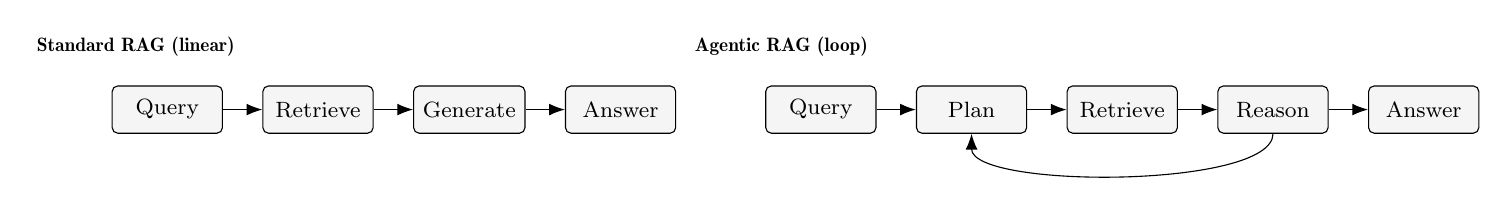
\begin{tikzpicture}[
  font=\footnotesize,
  node distance=0.4cm and 0.5cm,
  box/.style={draw, rounded corners=2pt, minimum width=1.4cm, minimum height=0.6cm, align=center, fill=VeryLightGray},
  arr/.style={-{Latex[length=2mm]}}
]
  % Linear
  \node[font=\scriptsize\bfseries] at (-0.2, 1.5) {Standard RAG (linear)};
  \node[box] (q1) at (0.2, 0.7) {Query};
  \node[box, right=of q1] (r1) {Retrieve};
  \node[box, right=of r1] (g1) {Generate};
  \node[box, right=of g1] (a1) {Answer};
  \draw[arr] (q1) -- (r1);
  \draw[arr] (r1) -- (g1);
  \draw[arr] (g1) -- (a1);

  % Agentic
  \node[font=\scriptsize\bfseries] at (8.0, 1.5) {Agentic RAG (loop)};
  \node[box] (q2) at (8.5, 0.7) {Query};
  \node[box, right=of q2] (p2) {Plan};
  \node[box, right=of p2] (r2) {Retrieve};
  \node[box, right=of r2] (g2) {Reason};
  \node[box, right=of g2] (a2) {Answer};
  \draw[arr] (q2) -- (p2);
  \draw[arr] (p2) -- (r2);
  \draw[arr] (r2) -- (g2);
  \draw[arr] (g2) -- (a2);
  \draw[arr] (g2.south) .. controls +(0,-0.7) and +(0,-0.7) .. (p2.south);
\end{tikzpicture}
\end{center}

\begin{itemize}
\item \textbf{Lec.\ 9 (Agentic AI / Claude Code)} shows how Claude Code combines RAG with tool use for end-to-end research workflows. Today's pipeline is the building block.
\end{itemize}
\end{frame}

\begin{frame}{Summary: The Four-Step Pipeline + the Why}
\begin{enumerate}
\item \textbf{Chunk.} Split documents into self-contained, metadata-rich pieces.

\medskip
\item \textbf{Embed.} Map each chunk to a vector so semantically similar text lives nearby in $\mathbb{R}^d$.

\medskip
\item \textbf{Store \& Retrieve.} Use a vector DB (Chroma, Qdrant, FAISS) for local semantic search; add graph or hierarchical indexes when the task depends on relationships, coverage, or multi-hop reasoning.

\medskip
\item \textbf{Augmented Generation.} Insert the retrieved evidence into a prompt template that demands grounded, cited, refusable answers.
\end{enumerate}

\bigskip
\textbf{Why this matters:} A vanilla LLM hits a hard wall on freshness, scale, latency, cost, and attribution --- exactly the dimensions that matter most for academic research. RAG separates the cost of indexing from the cost of querying, giving you a system that is cheap to update, cheap to query, faithful to sources, and capable of refusing to answer.

\bigskip
\centering\emph{The LLM is the brain. The index is the memory. The retriever is the librarian.}
\end{frame}

\begin{frame}{Closing}
\begin{center}
\Large
RAG turns institutional text --- FOMC, NBER,\\
Congress, SEC, central banks --- into a\\
\textbf{queryable research instrument.}
\end{center}

\bigskip
\bigskip
\begin{itemize}
\item Today: the static pipeline. Build it once, query it for years.
\medskip
\item \textbf{Next lecture (Lec.\ 9):} how an agentic system (Claude Code) uses RAG as one tool among many, plans multi-step research workflows, and edits its own code along the way.
\end{itemize}

\bigskip
\centering\textbf{Questions?}
\end{frame}

\end{document}
